\chapter{Introdução}
\label{cap-introducao}

A gestão dos ativos (Asset Management) de uma organização seja ela pública ou privada, independente de sua finalidade, é cada vez mais adotada ao redor do mundo como uma ferramenta para enfrentar os desafios econômicos impostos por um mercado globalizado diversificado ou uma sociedade que exige do poder público maior transparência e eficiência no emprego de seus tributos, já que a administração eficiente dos ativos tem a capacidade de aperfeiçoar o desempenho técnico e econômico dos equipamentos, acelerar o retorno sobre os investimentos realizados, e colaborar com planejamento organizacional trazendo previsibilidade e controle dos gastos envolvidos. 

Dentre as áreas da gestão de ativo, a manutenção é geralmente encarada como uma despesa que se deseja ao máximo adiar, não sendo uma pratica suficientemente valorizada. Esta opinião é compartilhada devido ser a manutenção uma fonte de custo, que não acrescenta um valor perceptível ao cliente final do produto ou serviço prestado pela organização, e gera indisponibilidades momentâneas no uso de bens e recursos.
Todavia, inevitavelmente a ação do tempo e o uso fazem com que equipamentos e instalações se desgastem, e precisem periodicamente de reparos, regulagens e limpeza para continuarem operando eficientemente.

A necessidade de se ter uma gestão de manutenção efetiva está se tornando cada vez importante, isso porque  reduzir desperdícios e executar com eficiência os processos de uma organização, tem se tornado cada dia mais necessário. Sendo o maior fator que impulsiona decisões hoje o custo e o lucro, quanto se está gastando para produzir e quanto se está obtendo de lucro. É aí que a manutenção se faz importante, porque o custo de realizar uma manutenção regular pode se tornar muito pequeno quando comparado ao custo de uma interrupção na produção ou atividades suportadas por ativos que necessitem de manutenção.

Assim, pode se definir com sendo um dos principais propósitos da manutenção, assegurar que todos os equipamentos requeridos para produção estejam funcionando com 100 porcento de eficência o tempo todo, por meio de inspeções diárias e pequenos ajustes, os quais ajudarão na detecção de problemas menores, diminuindo a chance de esses problemas se tornarem maiores ou até incorrigíveis \cite{krar2009}. Krar ainda diz que para se atingir uma manutenção regular e efetiva, é preciso que haja participação de todos, desde os alto executivo até as pessoas do operacional.

Com o reconhecimento da importância de se empregar processos efetivos de manutenção nas organizações, surgiu nos anos setenta Associações de Manutenção, na Espanha, México e Portugal, que despertou o interesse em profissionais brasileiros pelos conceitos, métodos e tecnologias que essa área dispõe. Em 1938, no III Congresso Ibero-Americano de Manutenção, foi aprovada a proposta de uma entidade no Brasil. Foi fundada então, em 17 de outubro de 1984, a Associação Brasileira de Manutenção, mudando seu nome em 2012 para Associação Brasileira de Manutenção e Gestão de Ativos. No começo, a ABRAMAN só tinha representantes dos setores de petróleo, eletrecidade, siderugia e transportes. Mais tarde a associação ganhou aderência por parte de setores diversos, por exemplo, hoje em dia a ABRAMAN emite certificados MBA de gestão de ativos para Instituições de Ensino Superior, assim como para outros setores. 

Em 1983, o IBP (Instituto Brasileiro de Petróleo) criou um documento nacional para análise da situação da manutenção no Brasil, a responsibilidade da elaboração passou para ABRAMAN desde a criação da associação em 1984, que em 1993, aderiu aos moldes de apresentação e desenvolvimen da AEM (Associação Espanhola de Manutenção), o qual é mantido até os dias de hoje.  

O Documento Nacional - A Situação da Manutenção no Brasil, apresenta resultados de pesquisas realizadas bienalmente, desde 1985, com indicadores de performance da Manutenção e Gestão de Ativos, presentes nos principais setores de produtos e serviços que movimentam a economia brasileira. No site da ABRAMAN \cite{abraman}, onde constam essas informações, também relata que um dos insumos para o documento são pesquisas e levantamento de índices em áreas de enfoque como \emph{ Forma de Atuação, Nível Hierárquico, Pessoal Próprio, Quadro Técnico, Rotatividade e Contratação de Pessoal, Contratação e Conceito dos Serviços, Critérios na Contratação, Composição dos Custos, Aplicação dos Recursos - Pessoal, Qualidade na Manutenção, Custo por Faturamento, Disponibilidade Operacional, Idade Média, Valor de Estoque e Segurança Industrial}. O documento tem uma alta relevância por representar de forma detalhada uma análise da situação da função no Brasil. Tendo servido como fonte de dados para profissionais, estudantes, pesquisadores e gerentes de empresas.

Em uma de suas últimas pesquisas, no ano de 2013, a ABRAMAN revelou que o custo total da manutenção representou em média 4,69 porcento do faturamento bruto nas empresas brasileiras, perfazendo uma parcela significativa do PIB nacional, na verdade o valor mais alto dessa estatística desde o inicio da série histórica iniciada em 1995, conforme a Figura~\ref{custo_anual_2013}.

\graphicspath{{figuras/}}
\begin{figure}[h]
\centering
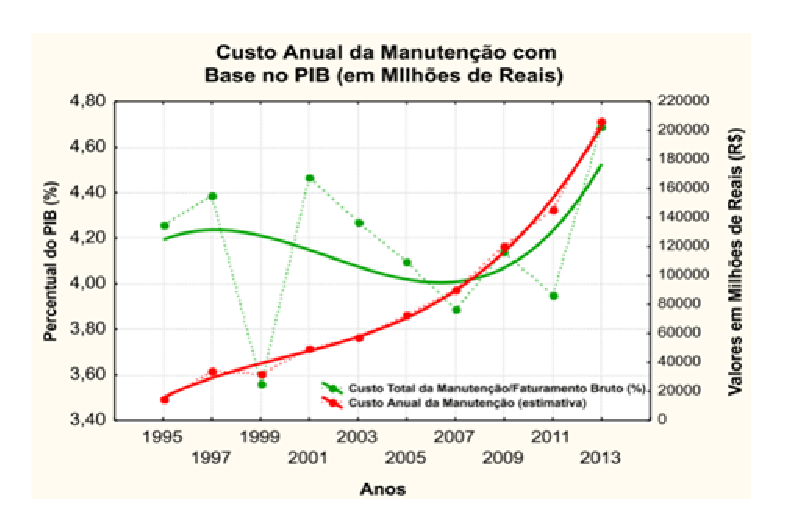
\includegraphics[width=0.8\textwidth]{dados_pib_pesquisa_intro.eps}
\caption{Custo anual da manutenção com base no PIB. \textbf{Fonte: ABRAMAN, Documento Nacional 2013.}}
\label{custo_anual_2013}
\end{figure}


Isto esta aliado ao que afirma DEKKER \cite{dekker1998} que relata que os gastos com manutenção tendem a crescer em todos os setores da economia, a despeito do desenvolvimento tecnológico, o que provocaria pensar que é uma contradição, porém as principais causas são a contínua expansão dos bens de capital e as exigências de mercado que impõe uma alta taxa de disponibilidade e confiabilidade dos equipamentos.

Dado essas informações, considerar a manutenção somente uma atividade operacional é não enxergar o valor significativo envolvido nessa área, nem sua responsabilidade para com a qualidade e imagem da organização. A função da manutenção deve possuir políticas e estratégias para que ela tenha a mesma relevância que outras funções da organização, atribuindo-lhe diretrizes e metas.	

No setor público as políticas de gestão da manutenção, como a de muitas outras áreas, tendem a evoluir em menor velocidade que na iniciativa privada, devido suas características legais e burocráticas que apesar de necessárias, para combater as praticas patrimonialistas, acabam por dificultar a inovação gerencial. Contudo o Estado precisa de um modelo de administração que traga resultados efetivos gastando a menor quantidade de recursos possíveis.

Neste contexto se insere o objeto de estudo deste trabalho: A universidade de Brasília – UnB. A qual segundo rankings nacionais, como o ENADE/MEC, e internacionais, como o \emph{Britanico Quacquarelli Symonds} (QS), se encontra entre as melhores do país e da América Latina, 10º e 9º lugar respectivamente. A Universidade possui grande importância por sua localização geográfica, capital do Brasil, e pesquisas desenvolvidas em diversas áreas de conhecimento, incluindo Engenharia e Saúde. Algumas destas pesquisas são realizadas em parceria com as melhores universidades do mundo, e induzem o denvolvimento do país, como por exemplo, a estação de monitoramento e correção diferenciada, que integra o \emph{Global Navigation Satellite System} (Glonass), em parceria com a Rússia, e as pesquisas na área da robótica desenvolvidas pelos departamentos de Engenharia de Software e Eletrônica da Universidade.

A UnB detém diversos laboratórios de pesquisa e certificação de alto valor e tecnologia, com um grande número de aparelhos e equipamentos científicos com sistemas complexos, todavia como outras instituições públicas de ensino superior, adotou políticas para a aquisição de um parque cientifico e tecnológico sem pensar em aspectos importantes para a manutenção, o que atrapalha os procedimentos em caso de defeitos, cometendo erro de não verificar a existência de meios humanos e materiais para a manutenção dos equipamentos, além disso, dispõe de processos de gestão de manutenções pouco informatizados, não possuindo indicadores de desempenhos claros que auxiliem seus gestores a tomada de decisão. Segundo (LIMA e CASTILHO, 2006) isso reflete, no caso particular da Universidade de Brasília, numa taxa de indisponibilidade exagerada dos equipamentos e instalações importantes para os laboratórios de ensino, pesquisa e de apoio administrativo, tendo como conseqüência a diminuição da capacidade produtiva da instituição e a insatisfação daqueles que dependem desse serviço.

Assim, a confiança nos serviços oferecidos pela Diretoria de Manutenção de Equipamentos – DIMEQ, unidade responsável por prover a manutenção e o reparo de equipamentos da Universidade, fica comprometida. 








%------------------------------------------------------------------------------%

\section{Problema}

Como melhorar a gestão da manutenção de equipamentos eletrônicos na UnB, por meio do desenho de uma solução que informatize-a, e apresente indicadores de desenpenho que auxilie seus gestores na tomada de decisões quanto ao tipo de manutenção que será aplicada a esses equipamentos ou quanto a substuição dele, levando em consideração o custo da escolha. 

%------------------------------------------------------------------------------%

\section{Justificativa}

O trabalho propõe melhorar a gestão da manutenção da UnB, tendo em vista que a má gestão da manutenção desperdiça recursos, trazendo gastos extras e não planejados, e também gera soluções precárias e tardias que elevam a taxa de indisponibilidade dos ativos, como os equipamentos eletroeletronicos e hospitalares. Além de que a má gestão pode diminuir o tempo de vida útil dos equipamentos tendo no caso particular da UnB, a consequência da diminuição da produção cientifica e da qualidade de ensido.

Em contrapartida, uma melhor gestão da manutenção maximiza a disponibilidade, confiabilidade e segurança dos equipamentos. O que traz maior previsibilidade dos custos, saindo da cultura do \lq\lq quebrou-concerta\rq\rq, atuando-se preventivamente. As falhas inesperadas diminuem fazendo com que o setor de manutenção contribua com o sucesso do negócio e não seja apenas um setor secundário ou de apoio, seja um setor consolidado que contribua ativamente com a melhoria da Universidade.



%------------------------------------------------------------------------------%

\section{Objetivo Geral}
 
O objetivo geral deste trabalho consiste na proposta de uma solução que informatize a gestão da manutenção de equipamentos eletrônicos da UnB, por meio da análise do seu ciclo de vida e da criação de modelos de manutenção na Seção~\ref{sec_modelos_manutencao} que possam melhor atender as necessidades de um certo tipo de equipamento. Assim como a realização de um estudao de caso, para validação da solução proposta. 

O estudo de caso consistirá na análise da recente decisão de se substituir o uso de projetores por televisões nas salas de aula da FGA, analisando as características de cada equipamento, seu ciclo de vida, confiabilidade, desempenho e custo.


%------------------------------------------------------------------------------%

\section{Objetivos Específicos}

Os objetivos específicos do trabalho são:

\begin{enumerate}
	\item Identificar falhas na gestão da manutenção de equipamentos eletrônicos da UnB, para sugerir melhorias, voltadas principalmente para a análise do ciclo de vida dos produtos.
	\item Sugerir uma solução que informatize dados importantes para a manutenção da Universidade, e forneça indicadores que auxiliem seus gestores na tomada de decisões.
	\item Simular a aplicação dos indicadores da manutenção através de um software interativo de cálculo numérico (MATLAB) 
	\item Validar solução por meio de um estudo de caso.
	\item Apresentar e descrever normas que padronizem a manutenção e gestão de ativos.
\end{enumerate}

%







